\section{Problem Statement}



\begin{frame}{Problem Statement}
 
\begin{block}{Distributed Monitors}
 
Let $\monitor = \{M_1, M_2, \ldots, M_n\}$ be a set of \Def{distributed 
monitors} monitoring an underlying system. 

\iffalse
Suppose $\alpha = s_0 s_1\cdots s_k$ is a finite trace 
generated by the system under inspection, and $\varphi$ is an \LTL formula.

\ \\

%\pause

Each monitor $M_i \in \monitor$ takes a sample \Def{only once} from the 
underlying system to obtain the values of propositions in $\AP$ as input.
\fi
\end{block}

\vspace{-10mm}
\begin{figure}
 \centering
 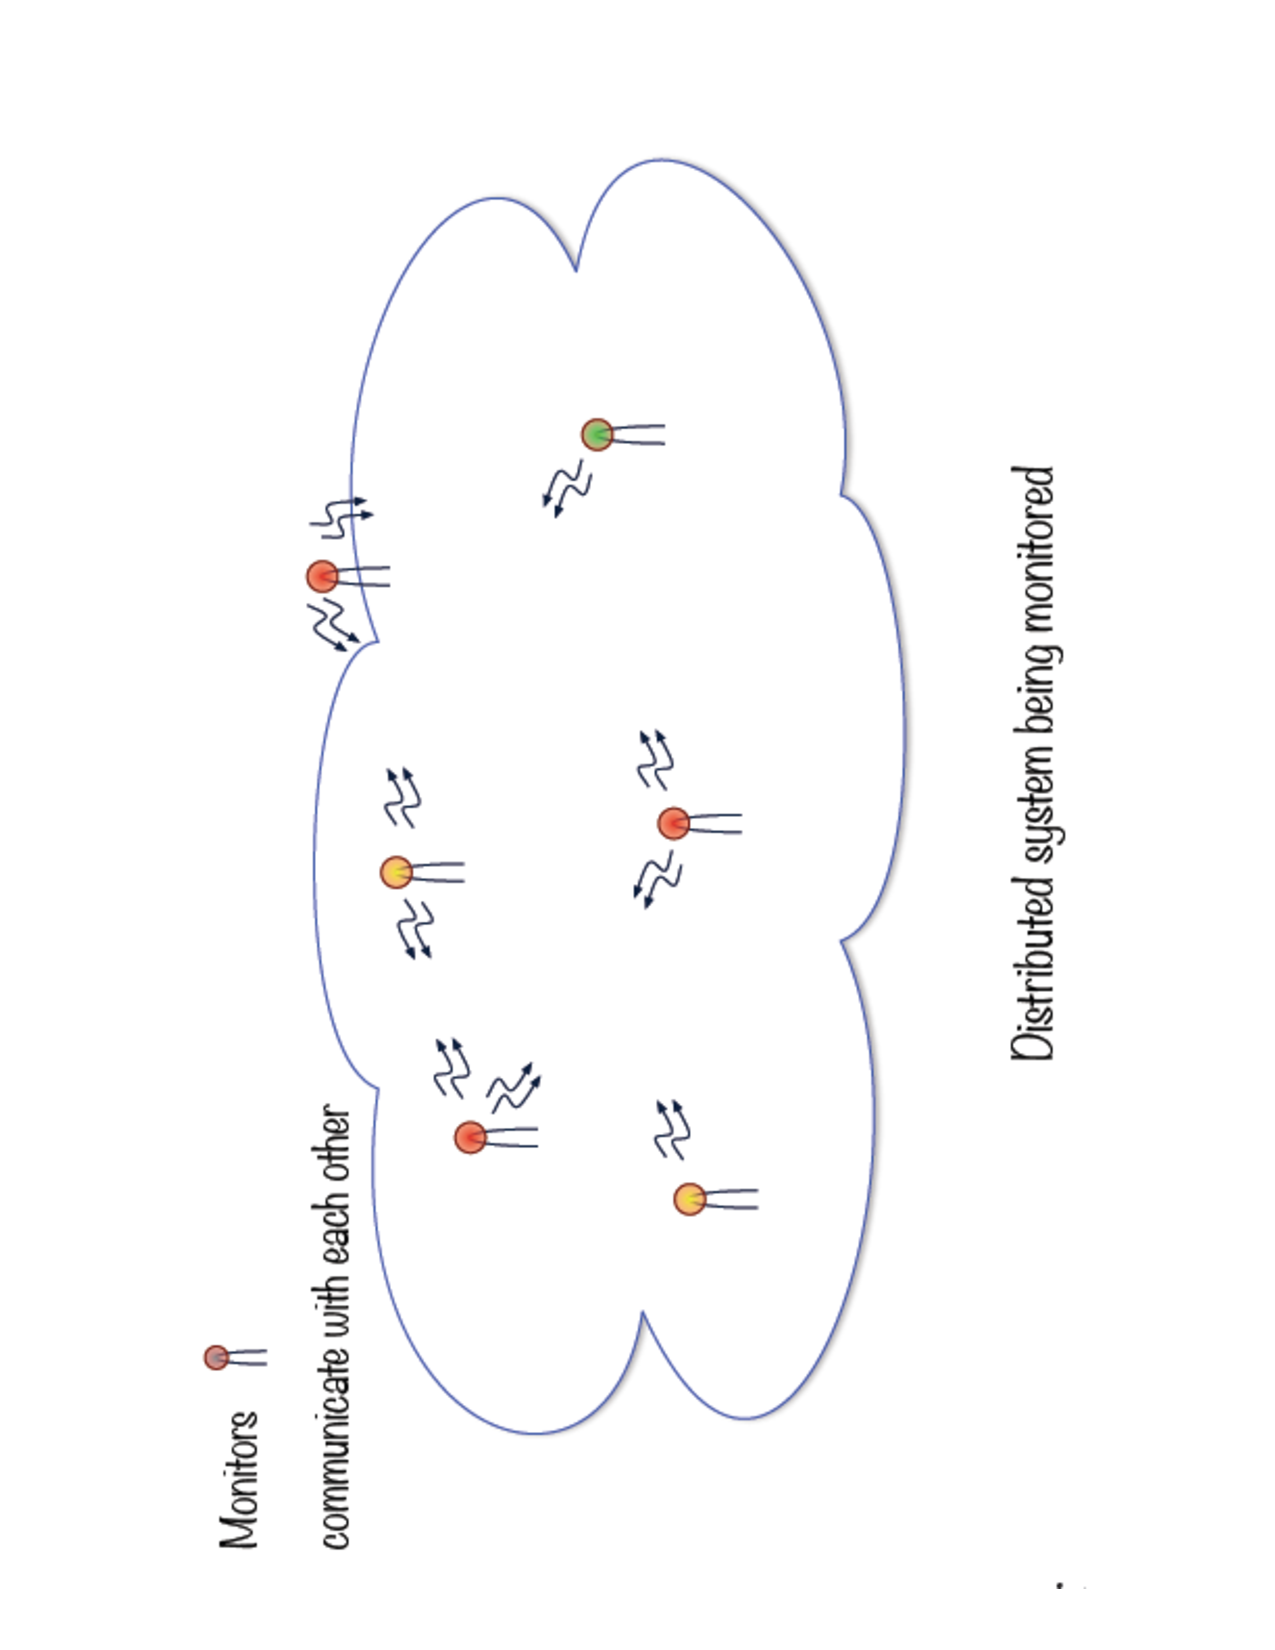
\includegraphics[scale=.29, angle=-90]{figures/wfdm}
 \end{figure}

\end{frame}
 
 % ----------------------------------------------------------------------------



\iffalse
\begin{frame}{Problem Statement}


\begin{block}{Synchronous Monitoring}

Let $\alpha = s_0 s_1\cdots s_k$ be a finite trace 
generated by the system under inspection, and $\varphi$ be an \LTL formula.

A non-faulty monitor should compute and emit a verdict that a centralized monitor that has global view of the system would compute. Formally:

$$\forall i \in [1, n] : M_i~ \text{is non-faulty} \; \rightarrow \valuation_i 
= [\alpha \models_3 \varphi]$$ 

\end{block}
\end{frame}
\fi




\begin{frame}{Synchronous Monitoring}

\begin{block}{Local Monitor Algorithm}
%\vspace{-15mm}

\begin{figure}
 \centering
 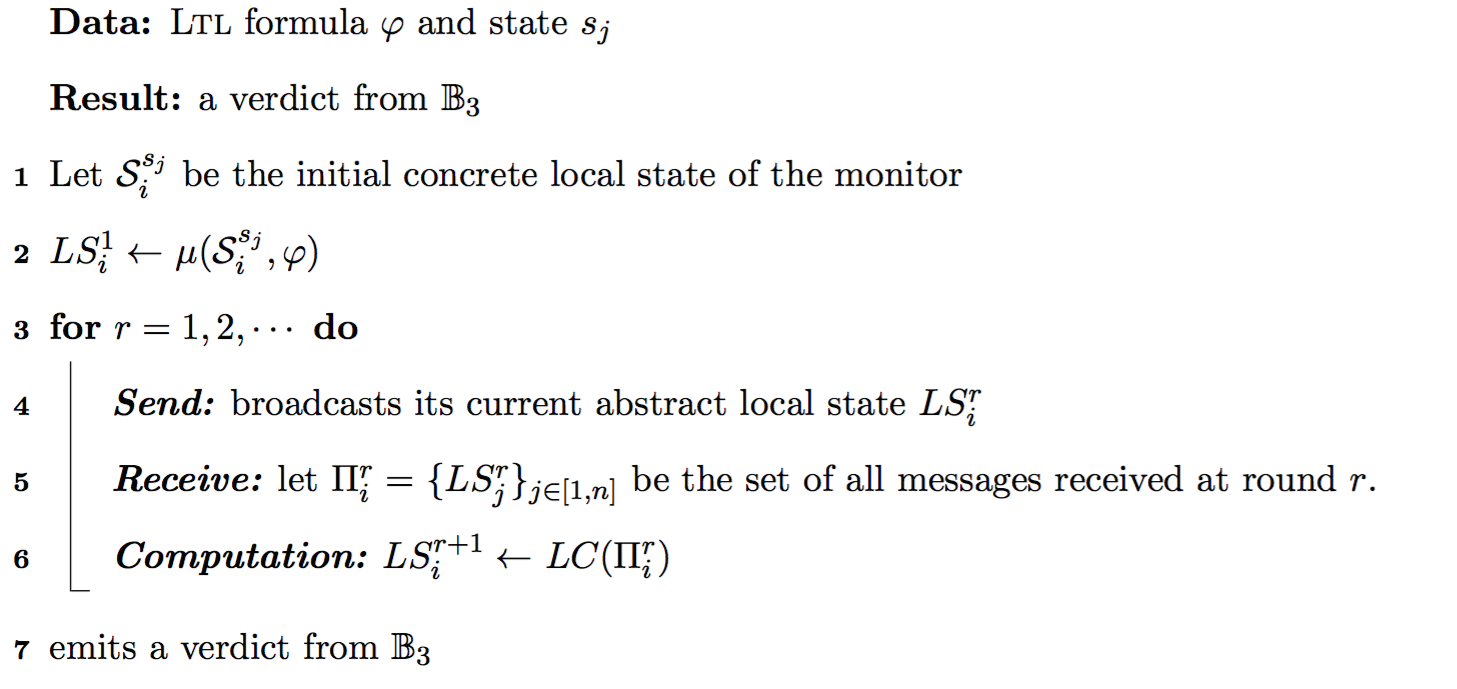
\includegraphics[scale=.3, angle=-360]{figures/synchalgo}
 \end{figure}
 
\begin{block}{Problem Statement}
A non-faulty monitor should compute and emit a verdict that a centralized monitor that has global view of the system would compute. Formally:

$$\forall i \in [1, n] : M_i~ \text{is non-faulty} \; \rightarrow \valuation_i 
= [\alpha \models_3 \varphi]$$ 

\end{block}

\end{block}

 \end{frame}
% ----------------------------------------------------------------------------








\iffalse

Suppose $\fintrace = \state_0\state_1\cdots \state_k$ is a finite trace 
generated by the system under inspection, and $\varphi$ is an \LTL formula with 
respect to which we monitor the system. Each monitor $M_i \in \monitor$, $i \in 
[1, n]$, runs Algorithm \ref{alg:localmonalgo} as follows. For any given new 
state $s_j$, monitor $M_i$ first obtains an initial concrete local state by 
taking a sample from $s_j$ (cf. Line 1). Recall from Definition 
\ref{def:concretestate} that the value of an atomic proposition in a 
concrete local state is either $\tru$, $\fals$, or $\natural$. After obtaining 
the initial concrete local state, monitor $M_i$ computes the initial local 
state based on the initial concrete local state (cf. Line 2). After 
intialization, each monitor $M_i$ executes a sequence of send, receive, and 
computation actions (cf. Lines 4-6) for some a priori known number of rounds.  
In Line 4, monitor $M_i$ sends its current abstract local state to all other 
monitors in $\monitor$. In Line 5, it receives messages from other monitors and 
stores them (along with its own message) in a set $\Pi_i^r$. In line 6, which is 
the computation step, monitor $M_i$ computes and updates its abstract local 
state based on messages in $\Pi_i^r$. Finally, after a certain number of rounds, 
the for-loop ends, and $M_i$ evaluates $\varphi$ and emits a \truthvalue~from 
$\mathbb{B}_3$ based on its final abstract local state (cf. Line 7). Note that 
Algorithm \ref{alg:localmonalgo} is executed whenever a new global state is 
reached in $\fintrace$. 

Our formal problem statement is the termination requirement for Algorithm 
\ref{alg:localmonalgo}. Roughly speaking, we require that when a 
non-faulty monitor runs Algorithm~\ref{alg:localmonalgo} to the end, it should 
compute and emit a verdict that a centralized monitor that has global view of 
the system would compute. This termination condition is formally, the following
$$\forall i \in [1, n] : M_i~ \text{is non-faulty} \; \rightarrow \valuation_i 
= [\alpha \models_3 \varphi]$$ 
where $\valuation_i$ is the \truthvalue~emitted by monitor $M_i$ at the end of 
running Algorithm~\ref{alg:localmonalgo}.


\fi


